% Method draft. Generated by make_paper_text.py -- do not edit numbers by hand.
\section{Method}
\label{sec:method}

Figure~\ref{fig:method} shows the pipeline as built: every path is run once on every query and cached, routers are
trained on the cached outcomes, and the trained router dispatches queries on a GPU pool at serving time.

\begin{figure*}[t]
  \centering
  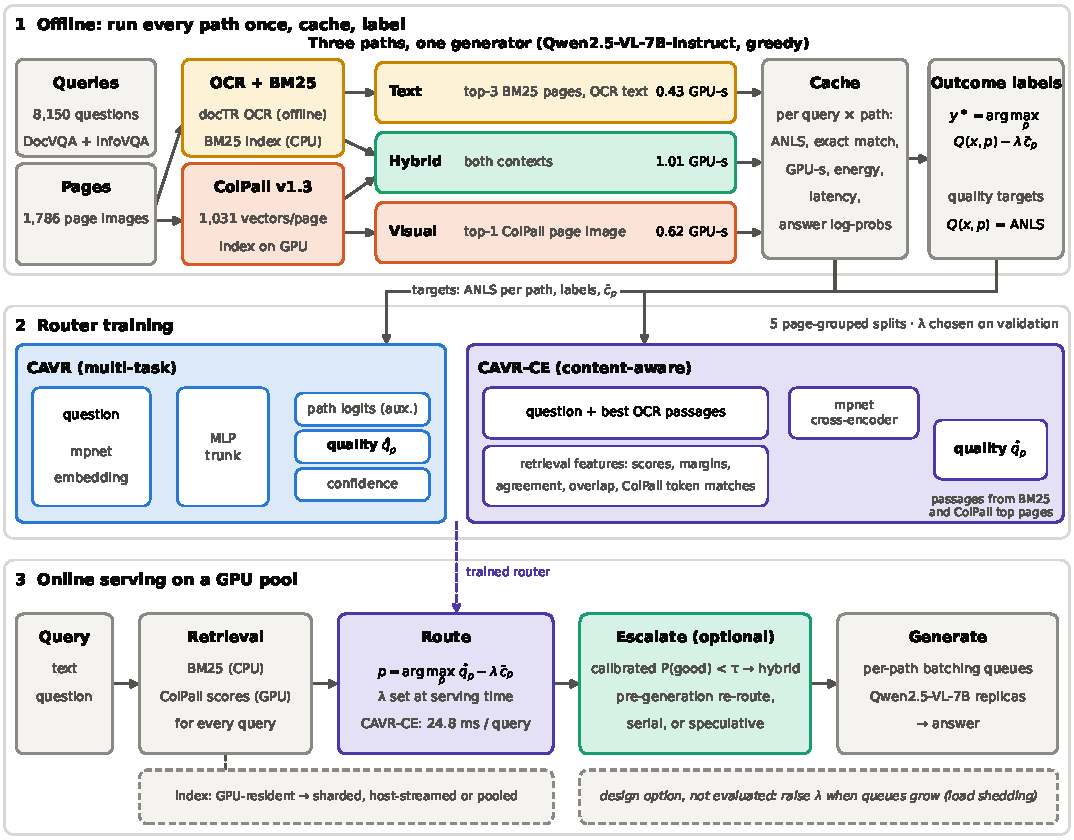
\includegraphics[width=\textwidth]{figures/method.pdf}
  \caption{CAVR as built. (1) Offline, every query is answered by all three paths with one shared generator; answer
  quality and measured cost are cached and turned into outcome labels (costs shown are mean GPU-seconds per query).
  (2) Two routers are trained on page-grouped splits: CAVR on the question embedding, and the content-aware CAVR-CE
  on the retrieved passages and retrieval features. (3) At serving time the router picks the path that maximises
  predicted quality minus $\lambda$ times its mean cost, optionally escalates to the hybrid path, and dispatches the
  query to per-path batching queues on the GPU pool. Dashed boxes are deployment options; load-adaptive $\lambda$ is
  not evaluated.}
  \label{fig:method}
\end{figure*}

\subsection{Problem formulation}
\label{sec:method-formulation}

Let $\mathcal{P} = \{\text{text}, \text{visual}, \text{hybrid}\}$ be the answer paths. For a query $x$ and path
$p$, let $Q(x,p) \in [0,1]$ be the quality of the answer (ANLS~\cite{anls}) and $c(x,p) \ge 0$ its cost
(GPU-seconds). A router only sees features $z(x)$ available before generation (the question and retrieval results).
A policy $\pi$ maps $z$ to a distribution $\pi(\cdot \mid z)$ over paths. Budget-constrained routing over a finite set
of queries $x_1,\dots,x_N$ is
\begin{equation}
  \max_{\pi}\; \frac{1}{N}\sum_{i}\sum_{p} \pi(p \mid z_i)\, Q(x_i,p)
  \quad\text{s.t.}\quad \frac{1}{N}\sum_{i}\sum_{p} \pi(p \mid z_i)\, c(x_i,p) \le B ,
  \label{eq:constrained}
\end{equation}
which is feasible when $B \ge \frac{1}{N}\sum_i \min_p c(x_i,p)$. Its Lagrangian is
$\mathcal{L}(\pi,\lambda) = \frac{1}{N}\sum_i \sum_p \pi(p\mid z_i)\,[Q(x_i,p) - \lambda c(x_i,p)] + \lambda B$
with $\lambda \ge 0$, and for a fixed $\lambda$ it is maximised query by query by the deterministic rule
\begin{equation}
  \pi_\lambda(z) = \arg\max_{p\in\mathcal{P}}\; \mathbb{E}[Q \mid z,p] - \lambda\, \mathbb{E}[c \mid z,p] .
  \label{eq:rule}
\end{equation}
Problem (\ref{eq:constrained}) is a linear program in the routing probabilities, so strong duality holds whenever it is
feasible: there is a $\lambda^\ast$ such that $\pi_{\lambda^\ast}$ is optimal once ties at $\lambda^\ast$ are
randomised with the probability that makes the budget bind. With one coupling constraint, a basic optimal solution
routes at most one query fractionally, so the best deterministic policy is within $1/N$ of the randomised optimum. A
sweep over $\lambda$ reaches the vertices of the upper convex hull of achievable cost--quality points; this sweep is
how we report the trade-off. The same Lagrangian form underlies cost-aware routers and cascades for language
models~\cite{frugalgpt,routellm}; here it is applied to context modalities that share one generator.

The submitted version maximised the ratio $Q/c$, which is not equivalent: the ratio ignores the budget. Consider
two paths with $(Q,c) = (0.50, 0.40)$ and $(0.60, 0.60)$. The ratio rule always picks the first (1.25 vs 1.00).
Under a budget $B \ge 0.60$ the constrained optimum is the second ($\lambda^\ast = 0$), and (\ref{eq:rule}) picks it
for every $\lambda < 0.5$.

\paragraph{Approximations used in practice.} Routers estimate $\mathbb{E}[Q \mid z,p]$ by a learned $\hat{q}_p(z)$.
For cost they use the mean cost of each path $\bar{c}_p$, estimated on the training split, in place of
$\mathbb{E}[c \mid z,p]$: per-query cost varies by 20--37\% (coefficient of variation) within
a path, mostly with output length, and is known exactly only after the query runs. Whether a budget is met is always
evaluated with the measured per-query costs. Outcome labels also use $\bar{c}_p$; the per-query oracle uses the true
per-query cost.

\subsection{Answer paths}
\label{sec:method-paths}

All paths share one generator, Qwen2.5-VL-7B-Instruct~\cite{qwen25vl}, with greedy decoding (the model's default repetition
penalty of 1.05 is kept) and at most 32 output tokens, so that cost differences come from the context
alone. Retrieval searches each dataset's own page pool.
\emph{Text}: BM25 over docTR~\cite{doctr} OCR text; the top 3 pages are given to the generator as text,
each cut to its first 2,000 characters. The cap keeps the longest prompts within GPU memory; it truncates
27\% of pages (44\% of InfographicVQA pages).
\emph{Visual}: ColPali v1.3~\cite{colpali} retrieves the top page by MaxSim over its patch vectors; the page image is
given to the generator at no more than 1280 visual tokens.
\emph{Hybrid}: the visual page image and the text context together.

\subsection{Cost model}
\label{sec:method-cost}

Every path is run once on every query on a single GPU at batch size 1, and the outputs are cached. Per query and path
we record GPU-seconds (generation plus, for paths that use it, ColPali query encoding and scoring), GPU energy from
NVML counters, peak GPU memory, and wall-clock latency including preprocessing and BM25 retrieval on the CPU. Router
overhead is measured separately and added to every routed query. When a router reads ColPali scores, ColPali
retrieval is charged to every query, including those routed to the text path, and never twice for the same query.
Offline costs (OCR, ColPali indexing) are reported separately. No cost is priced from list prices.

\subsection{Outcome-based labels}
\label{sec:method-labels}

The label of a query is the path that maximises $Q(x,p) - \lambda \bar{c}_p$, with ties broken towards the cheaper
path. We also report a threshold label: the cheapest path with ANLS $\ge$ 0.5, or the cheapest path when none
reaches it. Labels change with $\lambda$, so CAVR's decision rule uses its quality head; the label trains only an
auxiliary classification head.

\subsection{Routers}
\label{sec:method-routers}

\paragraph{CAVR.} A multi-task MLP over the all-mpnet-base-v2~\cite{mpnet,sbert} question embedding and a one-hot
dataset indicator, with hidden layers of 256 and 128 units (dropout 0.2) and three heads: path logits
(cross-entropy on the outcome label at $\lambda = 0.1$), per-path predicted quality $\hat{q}_p$ (squared error on
ANLS), and a confidence head (binary cross-entropy on whether the chosen path reaches ANLS $\ge$ 0.5), with loss
weights 1, 1 and 0.5. It is trained with AdamW (learning rate 0.001, weight decay 0.0001, batch 128),
with early stopping on validation utility at $\lambda = 0.1$ (patience 10 epochs).

\paragraph{CAVR-CE.} A content-aware quality predictor that reads what retrieval returned before any generation.
OCR text of each page is split into windows of 50 words with a stride of 25, and the windows most similar
to the question under the mpnet bi-encoder are selected: two from the BM25 top page, two from the ColPali top page and
one from each of BM25 pages 2--3, interleaved by importance. An mpnet cross-encoder reads the question paired with these
passages, truncated to 512 tokens (47\% of inputs are truncated, which mostly drops the lower-ranked
windows). Its pooled output is concatenated with standardised tabular features: BM25 and ColPali top scores and margins,
agreement and cross-ranks between the two retrievers, lexical and semantic overlap between the question and the
retrieved pages, OCR length, and ColPali per-token match statistics (for each question token, its best match on the top
pages). A two-layer head predicts $\hat{q}_p$ for every path, trained with binary cross-entropy against ANLS as a soft
target for 5 epochs (AdamW; learning rates 2e-05 for the encoder and 0.001 for the head; weight
decay 0.01; batch 16; linear warm-up and decay), keeping the epoch with the best validation AUC.

\paragraph{Choosing $\lambda$.} $\lambda$ is a run-time parameter. To report a single operating point without
tuning on test data, we choose on each split's validation set the cheapest $\lambda$ whose validation ANLS is within
0.005 of always-hybrid.

\subsection{Confidence-based escalation}
\label{sec:method-escalation}

A query routed to path $p$ is escalated to the hybrid path when a calibrated probability that its answer is good,
$g(x) = P(Q(x,p) \ge 0.5 \mid s(x))$, falls below a threshold $\tau$. The signals $s(x)$ are router confidence and
quality margin, retrieval scores and margins, and token log-probabilities of the generated answer; $g$ is fitted by
logistic regression on the validation split. Let $e(x) = \mathbb{1}[g(x) < \tau \wedge p \ne \text{hybrid}]$, let $L_r$
be router latency, $L^{\text{ret}}$ the latency of a set of retrievals, and $L^{\text{gen}}_p$ and
$c^{\text{gen}}_p$ the generation latency and GPU cost of path $p$. Each retrieval runs at most once per query and its
cost $c^{\text{ret}}$ is charged once. Per query:
\begin{align}
  \text{pre-generation re-route:}\quad & L = L_r + L^{\text{ret}}(R_0 \cup R_{p'}) + L^{\text{gen}}_{p'},
     \qquad p' = \text{hybrid if } e(x) \text{ else } p,\\
  \text{serial cascade:}\quad & L = L_r + L^{\text{ret}}(R_0 \cup R_p) + L^{\text{gen}}_p
     + e(x)\,\big[L^{\text{ret}}(R_{\text{hybrid}} \setminus R_0 \setminus R_p) + L^{\text{gen}}_{\text{hybrid}}\big],\\
  \text{speculative } (p \ne \text{hybrid}):\quad & L = L_r + L^{\text{ret}}(R_0 \cup R_{\text{hybrid}})
     + \max\big(L^{\text{gen}}_p, L^{\text{gen}}_{\text{hybrid}}\big),
     \quad c = c^{\text{gen}}_p + c^{\text{gen}}_{\text{hybrid}} + c^{\text{ret}},
\end{align}
where $R_0$ is the set of retrievals the signal itself needs and $R_p$ those path $p$ needs. Speculative execution
assumes two workers that do not interfere. We report p50 and p95 over the per-query values. Only pre-generation
signals avoid both the serial step and the doubled generation cost; answer-level signals require either a serial
cascade or speculative execution.

\subsection{Deployment on a GPU cluster}
\label{sec:method-deployment}

We envisage CAVR as a dispatcher in front of a GPU pool, with text retrieval on the CPU (Figure~\ref{fig:method},
band 3). BM25 retrieval, OCR text lookup and, optionally, the CAVR MLP run on CPU workers;
ColPali query encoding and scoring, CAVR-CE and generation run on GPUs, with one dynamic-batching queue per path. Our
load test models the GPU pool and its per-path queues; the dispatcher logic itself is not simulated. The visual index
is placed according to corpus size: GPU-resident while it fits, then sharded across GPUs, streamed from pinned host
memory, or pooled. Because $\lambda$ is a run-time input, the dispatcher could raise it when queues grow, shifting load
from the hybrid path to single-context paths instead of violating the latency target; we describe this option but do
not evaluate it.
